
%%%%%%%%%%%%%%%%%%%%%%%%%%%%%%%%%%%%%%%%%
% Short Sectioned Assignment
% LaTeX Template
% Version 1.0 (5/5/12)
%
% This template has been downloaded from:
% http://www.LaTeXTemplates.com
%
% Original author:
% Frits Wenneker (http://www.howtotex.com)
%
% License:
% CC BY-NC-SA 3.0 (http://creativecommons.org/licenses/by-nc-sa/3.0/)
%
%%%%%%%%%%%%%%%%%%%%%%%%%%%%%%%%%%%%%%%%%

\documentclass[paper=a4, fontsize=11pt]{scrartcl}
\usepackage[utf8]{inputenc}
\usepackage[spanish]{babel}
\usepackage{amsmath,amsfonts,amsthm}
\usepackage{sectsty}
\usepackage{fancyhdr}
\usepackage{sectsty}
\usepackage{graphicx}

\allsectionsfont{\textbf \normalfont}
\setlength\parindent{0pt}
\pagestyle{fancyplain}
\fancyhead{}
\fancyfoot[L]{Electrónica de Microondas}
\fancyfoot[C]{}
\fancyfoot[R]{\thepage}\fancyfoot[C]{}

\renewcommand{\headrulewidth}{0pt}
\renewcommand{\footrulewidth}{0pt}
\setlength{\headheight}{13.6pt}
\newcommand{\horrule}[1]{\rule{\linewidth}{#1}}
\newcommand{\exercisetitle}[1]{
\section{}
#1 \\[0.1cm]
\horrule{1pt}
}
\title{
\normalfont \normalsize
\huge Ejercicios Tema 3 \\
\horrule{2pt} \\[0.5cm]
}
\author{Luis Sánchez Velasco}
\date{\normalsize\today}

\begin{document}

\maketitle

\newcommand{\propconstant}[1]{
  \begin{equation*}
      \gamma = \sqrt{(R + j\omega L)(G + j \omega C)} #1
  \end{equation*}
}

\newcommand{\propconstantnoloss}[1]{
  \begin{equation*}
      \gamma =j\omega \sqrt{ L C} #1
  \end{equation*}
}

\newcommand{\impedance}[1]{
  \begin{equation*}
      Z_0 = \sqrt{\frac{(R + j\omega L)}{(G + j \omega C)}}  #1
  \end{equation*}
}

\newcommand{\impedancenoloss}[1]{
  \begin{equation*}
    Z_0 = \sqrt{\frac{L}{C}} #1
  \end{equation*}
}

\newcommand{\swr}[1]{
  \begin{equation*}
    SWR = \frac{1 + | \Gamma_L |}{1 - | \Gamma_L |} #1
  \end{equation*}

}

\exercisetitle{
Una línea de transmisión posee los siguientes parámetros por unidad de longitud: $L=0.3\mu H/m$, $C=450pF/m$,
$R=5\Omega /m$, y $G=0.01S/m$. Calcular la constante de propagación y la impedancia característica de esta
línea a $880MHz$. Recalcular estos parámetros en ausencia de pérdidas.}

La constante de propagación en medios con perdidas se define como:
\propconstant{ = \alpha + j \beta}
Donde sustituyendo por los valores dados en el ejercicio, $L=0.3\mu H/m$, $C=450pF/m$, $R=5\ohm /m$, y $G=0.01S/m$ obtenemos:
\begin{align*}
  \alpha &= 0.226 \\
    \beta &= 64.2
\end{align*}
Y para el cálculo de la impedancia característica:
\impedance{= 25.8 + 0.01j }
\\[0.5cm]
Para el caso sin perdidas asumiremos $R = G= 0$, por lo que la constante de propagación quedará como:
\propconstantnoloss{ = 64j}
y la impedancia característica:
\impedancenoloss{= 25.8 \Omega}

\exercisetitle{
Una línea de transmisión sin perdidas de longitud $0.3\lambda$ termina en una impedancia de carga, $Z_L$. Encontrar
el coeficiente de reflexión en la carga, el SWR de la linea y la impedancia de entrada de la linea. $(Z_0=75
\Omega, Z_L = 40 + j20 \Omega)$.
}
Para calcular primeramente el coeficiente de reflexión, situaremos en la carta de Smith el punto $z = \frac{40}{75} + \frac{20}{75}j \Omega$, marcado con un '1' en al gráfica. Donde observando el ángulo y la fase de este punto, obtenemos:
\[ \Gamma_L = 0.34e^{j2.45} \]

Para calcular el SWR haremos:
\swr{ \approx 2}

Para calcular la impedancia a la entrada moveremos el punto '1' $0.3 \lambda$ hacia el generador, punto '2' y observaremos que lineas corta. En este caso:
$z_i = 0.94 + 0.7i$ que al denormalizar quedará como: $Z_{in} = 67.5 + 52.5j$.

\begin{figure}[h]
  \centering
  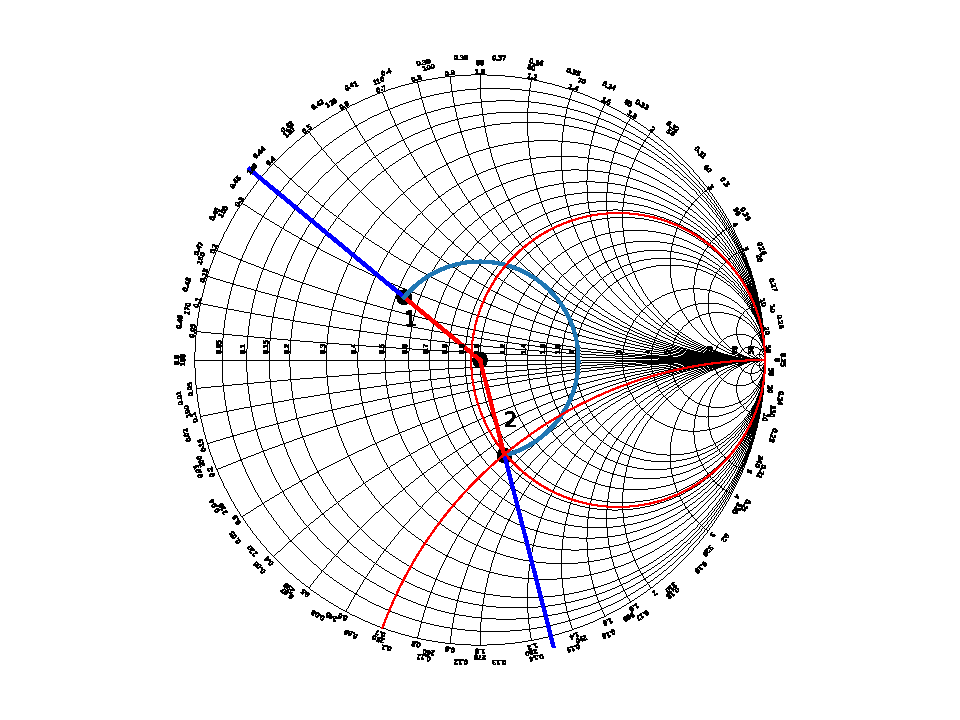
\includegraphics[scale = 0.85]{ej2/images/out.pdf}
  \caption{Moviendo el punto $0.3 \lambda$}
  \label{ej2smith}
\end{figure}

\exercisetitle{
Una línea de transmisión sin pérdidas de impedancia característica $Z_0$ se termina con una impedancia de
carga de $150 \Omega$.  Si se mide una SWR en la línea de 1.6, encontrar los dos posibles valores para $Z_0$.
}
Aunque el enunciado nos dice que existen dos posible valor para $Z_0$, solo existe uno, ya que tanto la impedancia de carga, como la de la línea (sin pérdidas), son reales.
Para resolverlo empezaremos evaluando la expresión del SWR:
\swr{ = 1.6}
Donde podemos resolver para $| \Gamma_L |$,obteniendo:
\[ | \Gamma_L | = 0.23 \]
Sabemos que al ser las dos impedancias puramente reales, el valor absoluto del coeficiente de reflexión será igual a su valor real, esto se puede observar en la expresión del coeficiente de reflexión en función de la impedancia de carga y la impedancia carcterística de la línea.

\reflectionfromimpedance{ = 0.23}

De donde podemos obtener $Z_0$, el cual resulta:
\[Z_0 = 93.9 \Omega \]

\exercisetitle{
Un transmisor wireless está conectado a una antena con impedancia de entrada de $80+j50\Omega$ a través de
un cable de $50\Omega$.  Si el transmisor de $50\Omega$ puede suministrar una potencia de 30W cuando se conecta a
una carga adaptada, ¿cuál es la potencia suministrada a la antena?  Repetir el cálculo suponiendo que el
transmisor tiene una impedancia de salida de $60\Omega$.
}

Nos encontramos on la situación en la que tenenemos una línea por la que circulan 30W, de los cuales el $100\%$ irán hacia la carga cuando esta este adaptada. Calcularemos que potencia irá hacia la carga en los siguientes casos:
\subsection{$Z_0 = 50\Omega$}
En este caso el coeficiente de reflexión será:
\reflectionfromimpedance{ = \frac{80+j50\Omega - 50\Omega}{80+j50\Omega + 50\Omega} = 0.418e^{j0.663} }
Y la potencia entregada:
\begin{align*}
  P_{in} &= P_{out}(1- \Gamma_L)
  P_{in} &= 30(1- 0.41)
  P_{in} &= 17.7 W
\end{align*}
\subsection{$Z_0 = 60\Omega$}
Repitiendo las cuentas:
\reflectionfromimpedance{ = \frac{80+j50\Omega - 60\Omega}{80+j50\Omega + 60\Omega} = 0.368e^{j1.533} }
Y la potencia entregada:
\begin{align*}
  P_{in} &= P_{out}(1- \Gamma_L)
  P_{in} &= 30(1- 0.368)
  P_{in} &= 18.96 W
\end{align*}

\exercisetitle{
Asumiendo que la impedancia característica es real, mostrar que para una carga puramente reactiva de
la forma $Z_L = jX_L$, la magnitud del coeficiente de reflexión es siempre la unidad.
}

Para demostrar esto empezaremos colocando la expresión del coeficiente de reflexión:
\[\Gamma_L = \frac{jX_L - Zo}{jX_L + Zo} \]
Y convertiremos tanto el divisor como el denominador a modulo y fase:
\begin{align*}
  \Gamma_L &= \frac{\sqrt{(X_L)^2 +(-Zo)^2]}e^{jarctan(\frac{X_L}{-Z_0} )}  }{\sqrt{(X_L)^2 +(Zo)^2]}e^{jarctan(\frac{X_L}{Z_0} )}  } \\
  \Gamma_L &= 1e^{j(\arctan{\frac{X_L}{-Z_0} } - \arctan{\frac{X_L}{Z_0} })}
\end{align*}
Como la función arcotangente es impar:
\[ \Gamma_L &= e^{-j2\arctan{\frac{X_L}{Z_0} }

Se puede ver como ambos modulos serían iguales, dividiendose los dos a 1, esto tiene sentido ya que si la caraga fuese puramente reactiva, no debería consumir ningún tipo de enrergía, por tanto toda ha de ser rebotada hacia el generador.

\exercisetitle{
Para  el  circuito  mostrado,  encontrar  la  potencia  transmitida  a  la  carga  y  la  potencia  disipada  en  el
generador para una impedancia de carga $Z_L= 30 +j40\Omega$.  ¿Qué valor de la impedancia de carga permitirá una entrega maxima de potencia a la carga?  ¿Cuál es esta potencia?

}
\subsection{$Z_L = 30 + 40 \Omega$}
Procederemos de la siguiente manera:
\begin{enumerate}
  \item Calcularemos la impedancia normalizada de la carga
  \item Situaremos esta impedancia en la carta de smith, obteniendo $\Gamma_L$
  \item Moveremos la línea $0.7\lambda$ hacia el generador para obtener $z_{in}$
  \item Denormalizaremos $z_{in}$ y obtenedremos la potencia entregada a la línea.
\end{enumerate}

\begin{figure}[h]
  \centering
  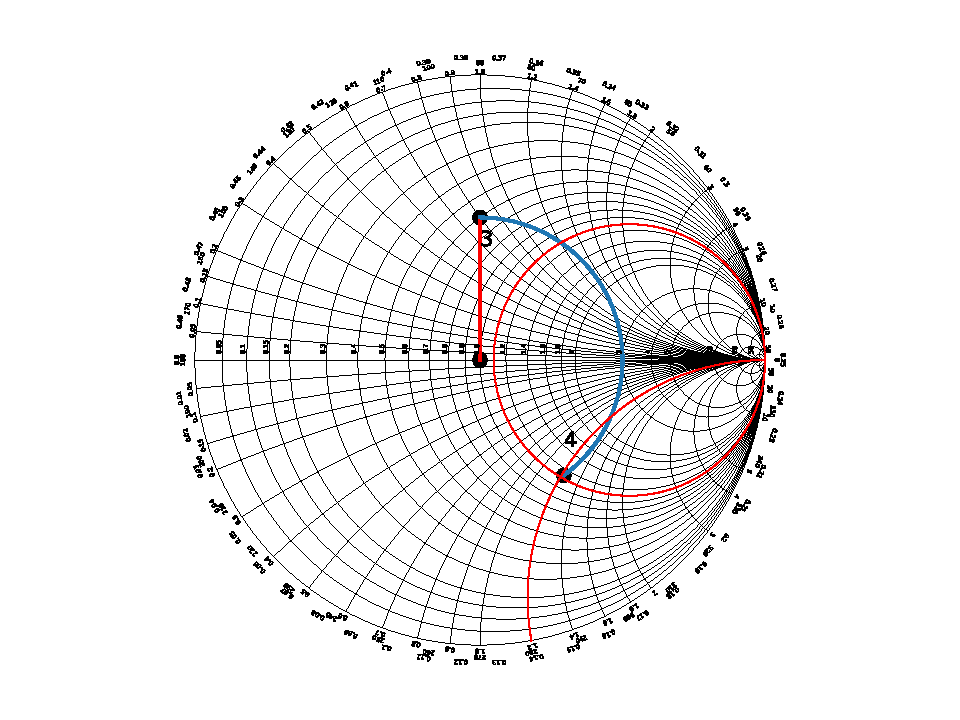
\includegraphics[scale = 0.85]{ej6/images/out1.pdf}
  \caption{Pasos 3 y 4}
  \label{ej2smith}
\end{figure}

En este caso $z_in = \frac{3}{5} + j\frac{4}{5}$, obteniendo, como se puede ver en la figura 2:
\[ \Gamma_L = 0.5e^{j1.57} \]
Tras mover la línea $0.7\lambda$ obtenemos $z_{in} = 1.1 + 1.2j$, que denormalizado queda como:
\[Z_{in} = 55 + 60j\]
 Con lo que podremos calcular la potencia de entrada a la línea con la siguiente expresión:
\begin{align*}
  P_{in} &= \frac{1}{2}|V_S|^2 \frac{R_{in}}{(R_S + R_{in} )^2 + (X_S + X_{in})^2}
  P_{in} &= \frac{1}{2}100  \frac{55}{(20+55)^2 + (30+60)^2}
  P_{in} &= 0.2 W
\end{align*}

Por lo tanto se entregarán 0.2W a la carga, ya que al no tener la línea perdidas, toda este energía se entregará a la carga.

\subsection{¿Qué valor de la impedancia de carga permitirá una entrega maxima de potencia a la carga?}
El valor que hará que esta potencia entregada a la carga sea máxima será el que haga que la impedancia de entrada a la línea sea: $Z_{in} = R_S - X_S$, por que empezaremos normalizando este valor con la impedancia del generador: $z_{in} = 0.4 + 0.6j$. Situaremos este valor en la carta de smith, y retrocederemos hasta la carga $0.7\lambda$, y la impedancia obtenida será la que máximize la potencia entregada  la carga.

\begin{figure}[h]
  \centering
  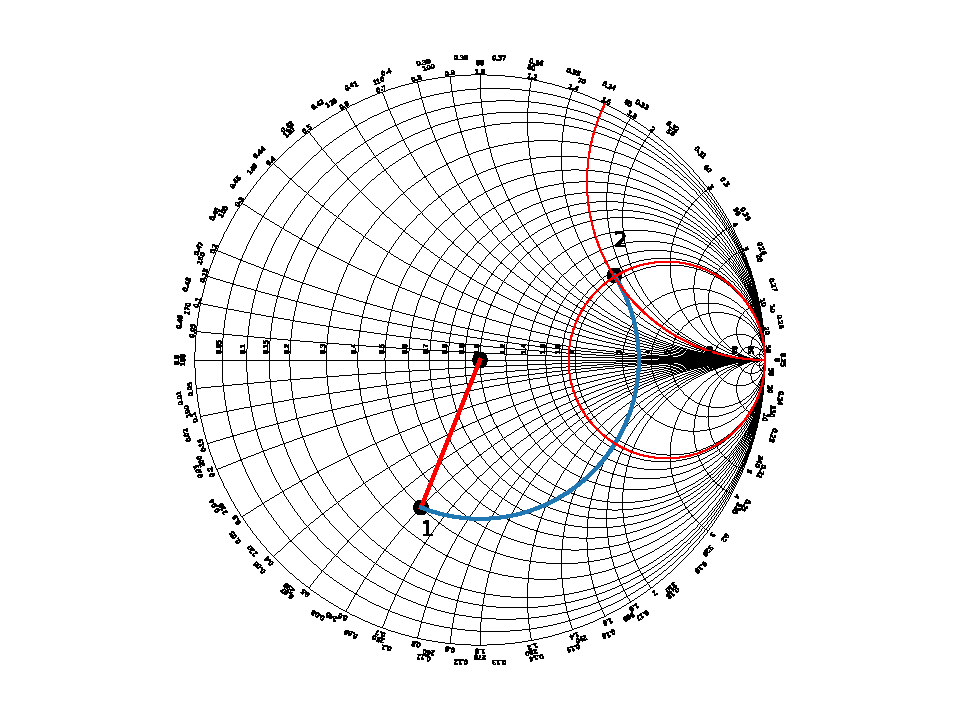
\includegraphics{ej6/images/out2.pdf}
  \caption{Avanzando $0.7\lambda$ hacia la carga}
  \label{ej2smith}
\end{figure}

Donde podemos ver que la impedancia normalizada $z_l = 1.9 +1.6j$, que denormalizada es $Z_L = 95 + 80j \Omega$

\subsection{¿Cuál es esta potencia?}
Podemos usar la expresión de la potencia entregada a la carga cuando la línea esta completamente adaptada a la línea:
\[P_{in} = \frac{|V_s|^2}{8R_s} = 0.625W\]

\exercisetitle{
En el circuito de la figura, usar la carta de Smith para encontrar el SWR de la línea, el coeficiente de reflexión en la carga, la admitancia de carga, la impedancia de entrada de la línea, la distancia desde la carga hasta el primer mínimo de voltaje, y la distancia desde la carga al primer máximo de voltaje.
}
Primero normalizaremos la impedancia en la carga como: $z_l = 1.4 + 0.8j$
\subsection{SWR y $\Gamma$}
Para calcular estos valores usando la carta de smith situamos la impedancia normalizada en la carta y medimos la distancia hasta el origen (0, 0),  usando las diferentes escalas en la parte de abajo podremos obtener los valores.
Estos valores resulta SWR = 2 y $\Gamma = 0.32$
\begin{figure}[h]
  \centering
  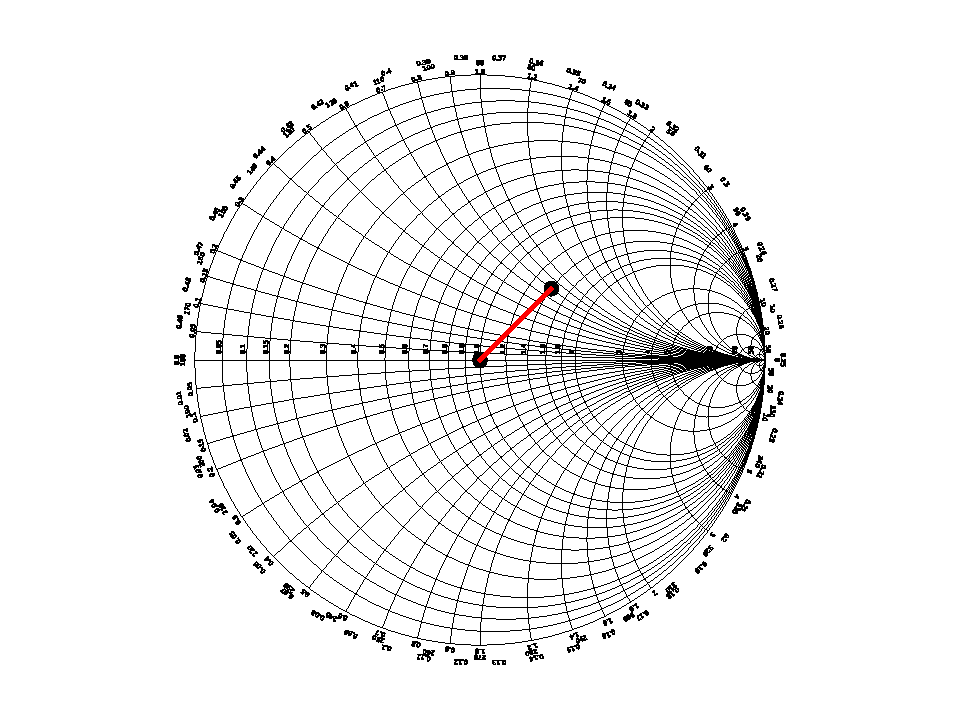
\includegraphics{ej7/images/out1.pdf}
  \caption{SWR y $\Gamma$}
  \label{ej2smith}
\end{figure}
\newpage
\subsection{Admitancia de la carga}
Para calcular la admitancia moveremos el punto anteriormente obtenido $180\º$ y denormalizaremos el mismo multiplicando por $\frac{1}{Y_0}$
\begin{figure}[h]
  \centering
  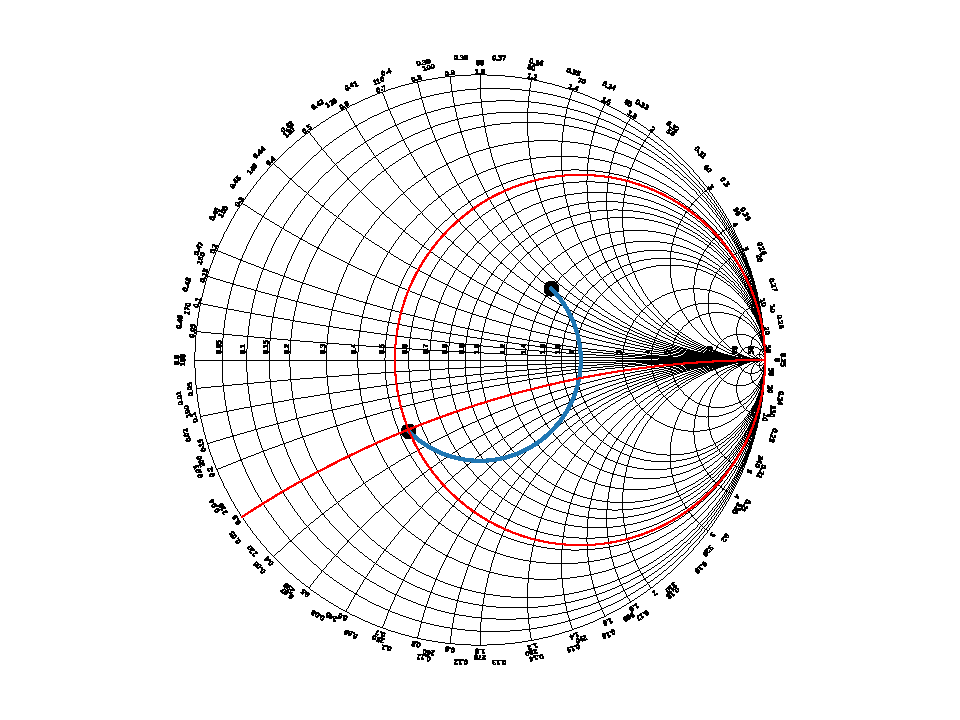
\includegraphics{ej7/images/out2.pdf}
  \caption{Admitancia}
  \label{ej2smith}
\end{figure}
\newline
Donde al denormalizar obtenemos $Y_l =  0.018 + j6 \times 10^{-3} S$
\newpage

\subsection{Impedancia de entrada}
Para hayar la impedancia de entrada simplemente moveremos el punto obtenido en primer apartado $0.8\lambda$ hacia el generado y denormalizaremos la impedancia

\begin{figure}[h]
  \centering
  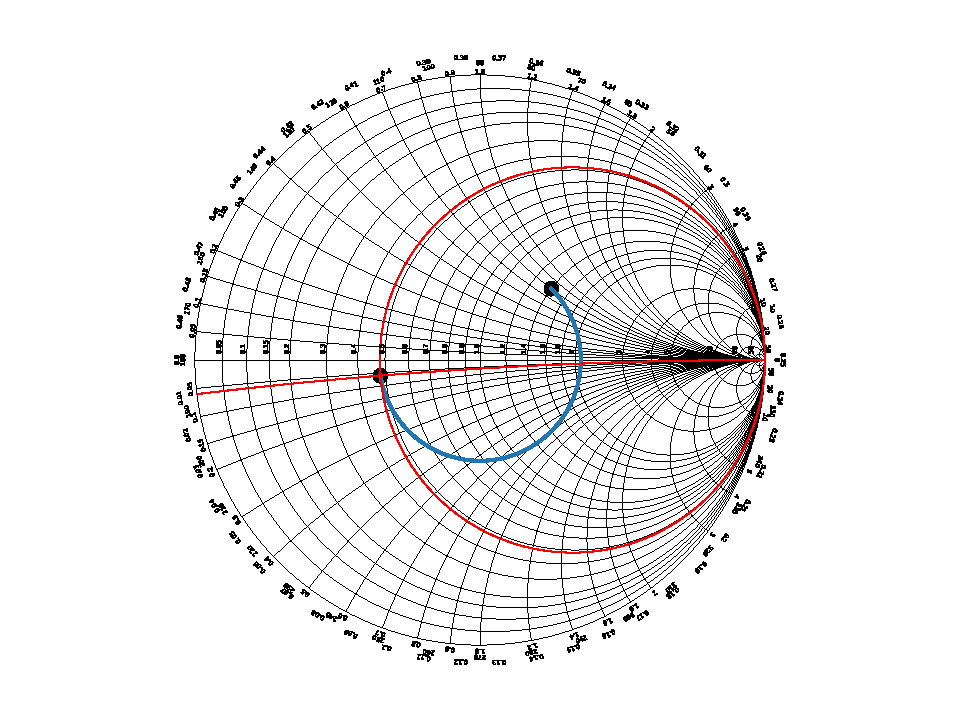
\includegraphics{ej7/images/out3.pdf}
  \caption{Impedancia de entrada}
  \label{ej2smith}
\end{figure}
Al denormalizar obtenemos $Z_{in} = 24 + 3j \Omega$
\newpage

\subsection{Máximo y mínimo}
Para hayar la distancia del primer máximo/mínimo nos fijaremos en el detalle de que los máximos y mínimos en la línea se producen cuando $Z(-l)$ es un número puramente real, por lo tanto la estrategia que seguiremos para hayar dichos puntos será avanzar el punto calculado en el apartado 1 hasta que la parte imaginaria sea 0, el siguiente máximo/minimo se encotrará a $\lambda / 4$ de este punto.
\begin{figure}[h]
  \centering
  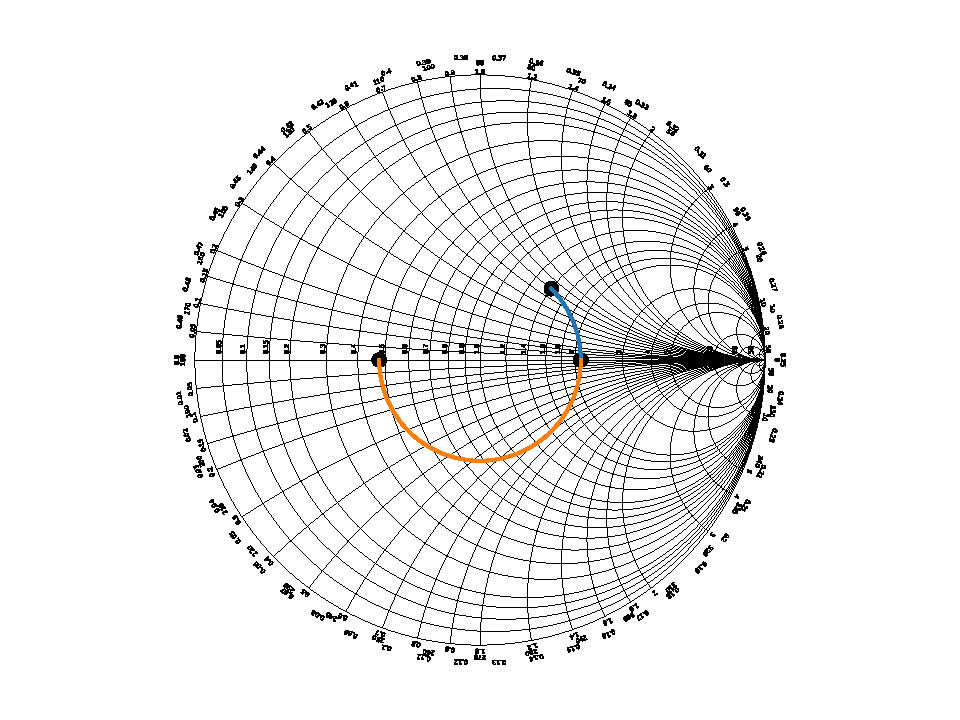
\includegraphics{ej7/images/out4.pdf}
  \caption{Máximo y mínimo}
  \label{ej2smith}
\end{figure}
Donde vemos que la distancia, en longitudes de onda, hasta el primer máximo ($Z_0 \leq Z(-l)$ ) es de $0.028\lambda$, por lo que el mínimo se encontrará a $0.278\lambda$.


\end{document}
